\chapter{Evaluation\label{evaluation}}

This chapter discusses how the changes implemented in chapter \ref{improvements} impact the performance of RIR.

For evaluation, the Shootout benchmarks were used. \todo

Additionaly, for testing things quickly during development, usually a kind of microbenchmark, such as the one in listing \ref{lst:microbench}, were checked by hand in fresh sessions of GNU R (with JIT disabled and with JIT set to 2) and RIR (with JIT enabled). In the code, a function is defined and measured repeatedly. The final reported time is computed as arithmetic mean of only a tailing part of the runs. This is to ensure a proper warmup (i.e. everything is byte-compiled by the JIT and possibly the processor branch predictors warm up).

\begin{listing}[htbp]
  \caption{\label{lst:microbench}Microbenchmark code}
  \begin{rcode}
f <- function() {
    i <- 10000000L
    while (i > 0) i <- i - 1
}
t <- c()
for (x in 1:10) t <- c(t, system.time(f())[[3]])
mean(t[5:10])
  \end{rcode}
\end{listing}

The scripts used to make the measurments can be found on the enclosed CD. \todo How was it measured? violet specs (i7, 8GB RAM)?

Figure \ref{fig:history} captures the running times of each benchmark over the course of the work described in chapter \ref{improvements}. The measurments were performed for some of the important revisions. Their list is also on the enclosed CD.

The revisions with short descriptions that were used to monitor the progress are listed in table \label{tab:git-rev}.

\begin{longtable}[c]{@{}ll@{}}
\caption{Git revisions used in the benchmarks\label{tab:git-rev}} \tabularnewline
\toprule
Hash & Description \tabularnewline
\midrule
\endfirsthead
\toprule
Hash & Description \tabularnewline
\midrule
\endhead
e1091b9 & \todo \tabularnewline
594af0c & \todo \tabularnewline
ce30085 & \todo \tabularnewline
6c4f526 & \todo \tabularnewline
f8e8238 & \todo \tabularnewline
12ef757 & \todo \tabularnewline
ff73d75 & \todo \tabularnewline
\bottomrule
\end{longtable}

\begin{figure}[htbp]
  \caption{\label{fig:history}History of running times}
  \centering
  \tmpframe{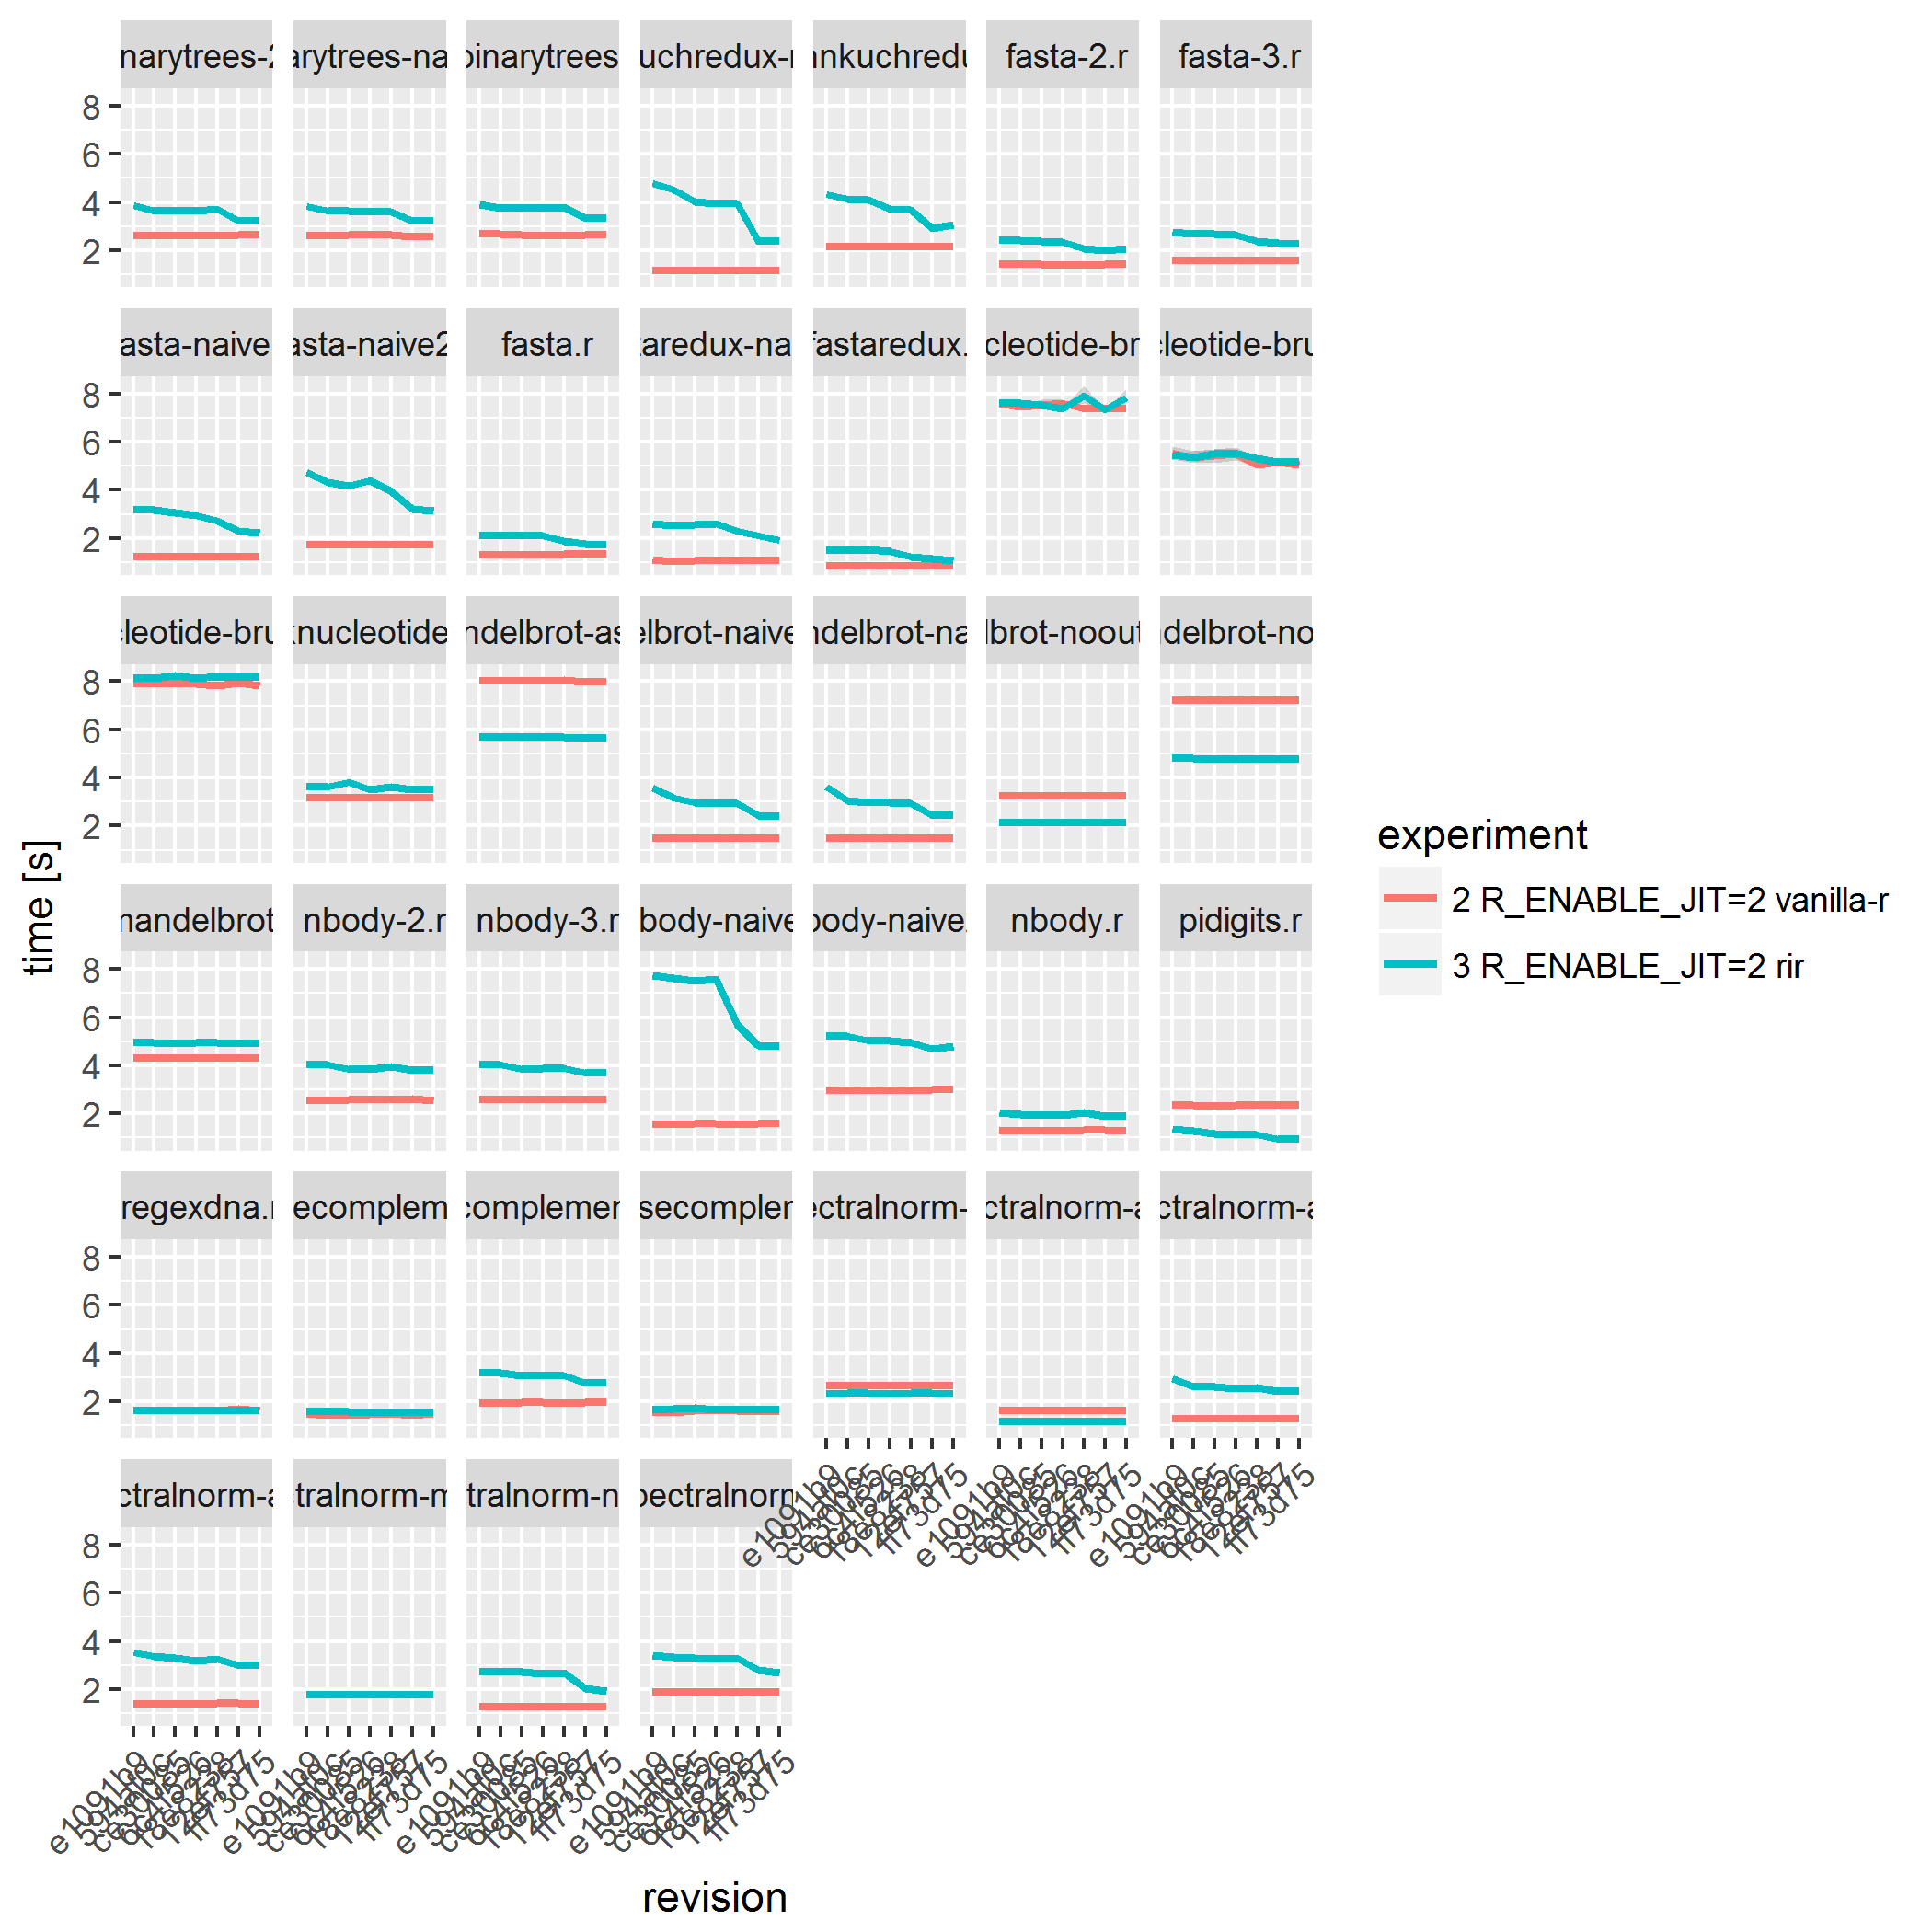
\includegraphics[width=\linewidth]{images/speedup_history}}
\end{figure}

In the figure, the light blue color represents the performance of the GNU R bytecode. As all measurments were carried out on the same version of GNU R (namely 3.3.2) the times should be constant over the history, and indeed they are.

For three mandelbrot, pidigits and two spectralnorm benchmarks RIR was already faster.

Knucleotide fastanaive some slowdowns.

Some mandelbrot, regexdna, spectralnorm, reversecomplement have not changed at all.

Nbody naive \todo[add plot] big drop interpreter refactoring. also fasta naive, fannkuchrecux naive, spectralnorm naive and others. describe what kind of code they are

Why pidigits so fast and why it improved further

The average speedup versus GNU R over the measured revisions is captured in figure \ref{fig:avg-speedup-history}.

\begin{figure}[htbp]
  \caption{\label{fig:avg-speedup-history}History of average speedup vs. GNU R}
  \centering
  \tmpframe{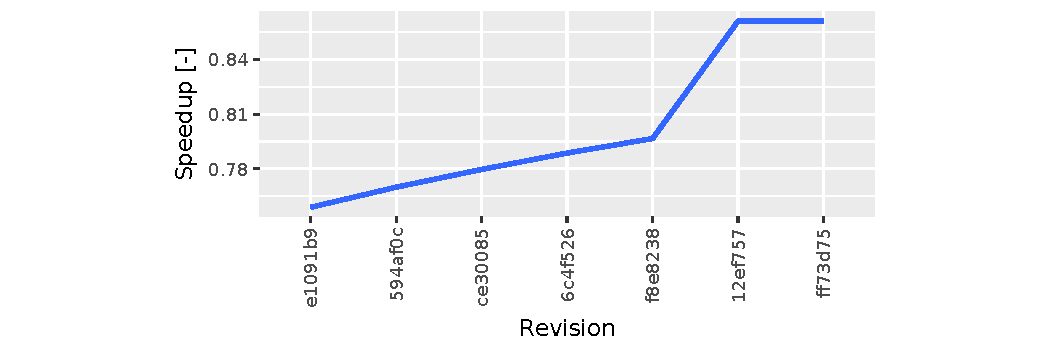
\includegraphics[width=\linewidth]{images/avg_speedup}}
\end{figure}

Figure \ref{fig:overall} shows the summary of speedups gained for all benchmarks, as well as an overall average speedup.

\begin{figure}[htbp]
  \caption{\label{fig:overall}Overview of the slowdown vs. GNU R}
  \centering
  \tmpframe{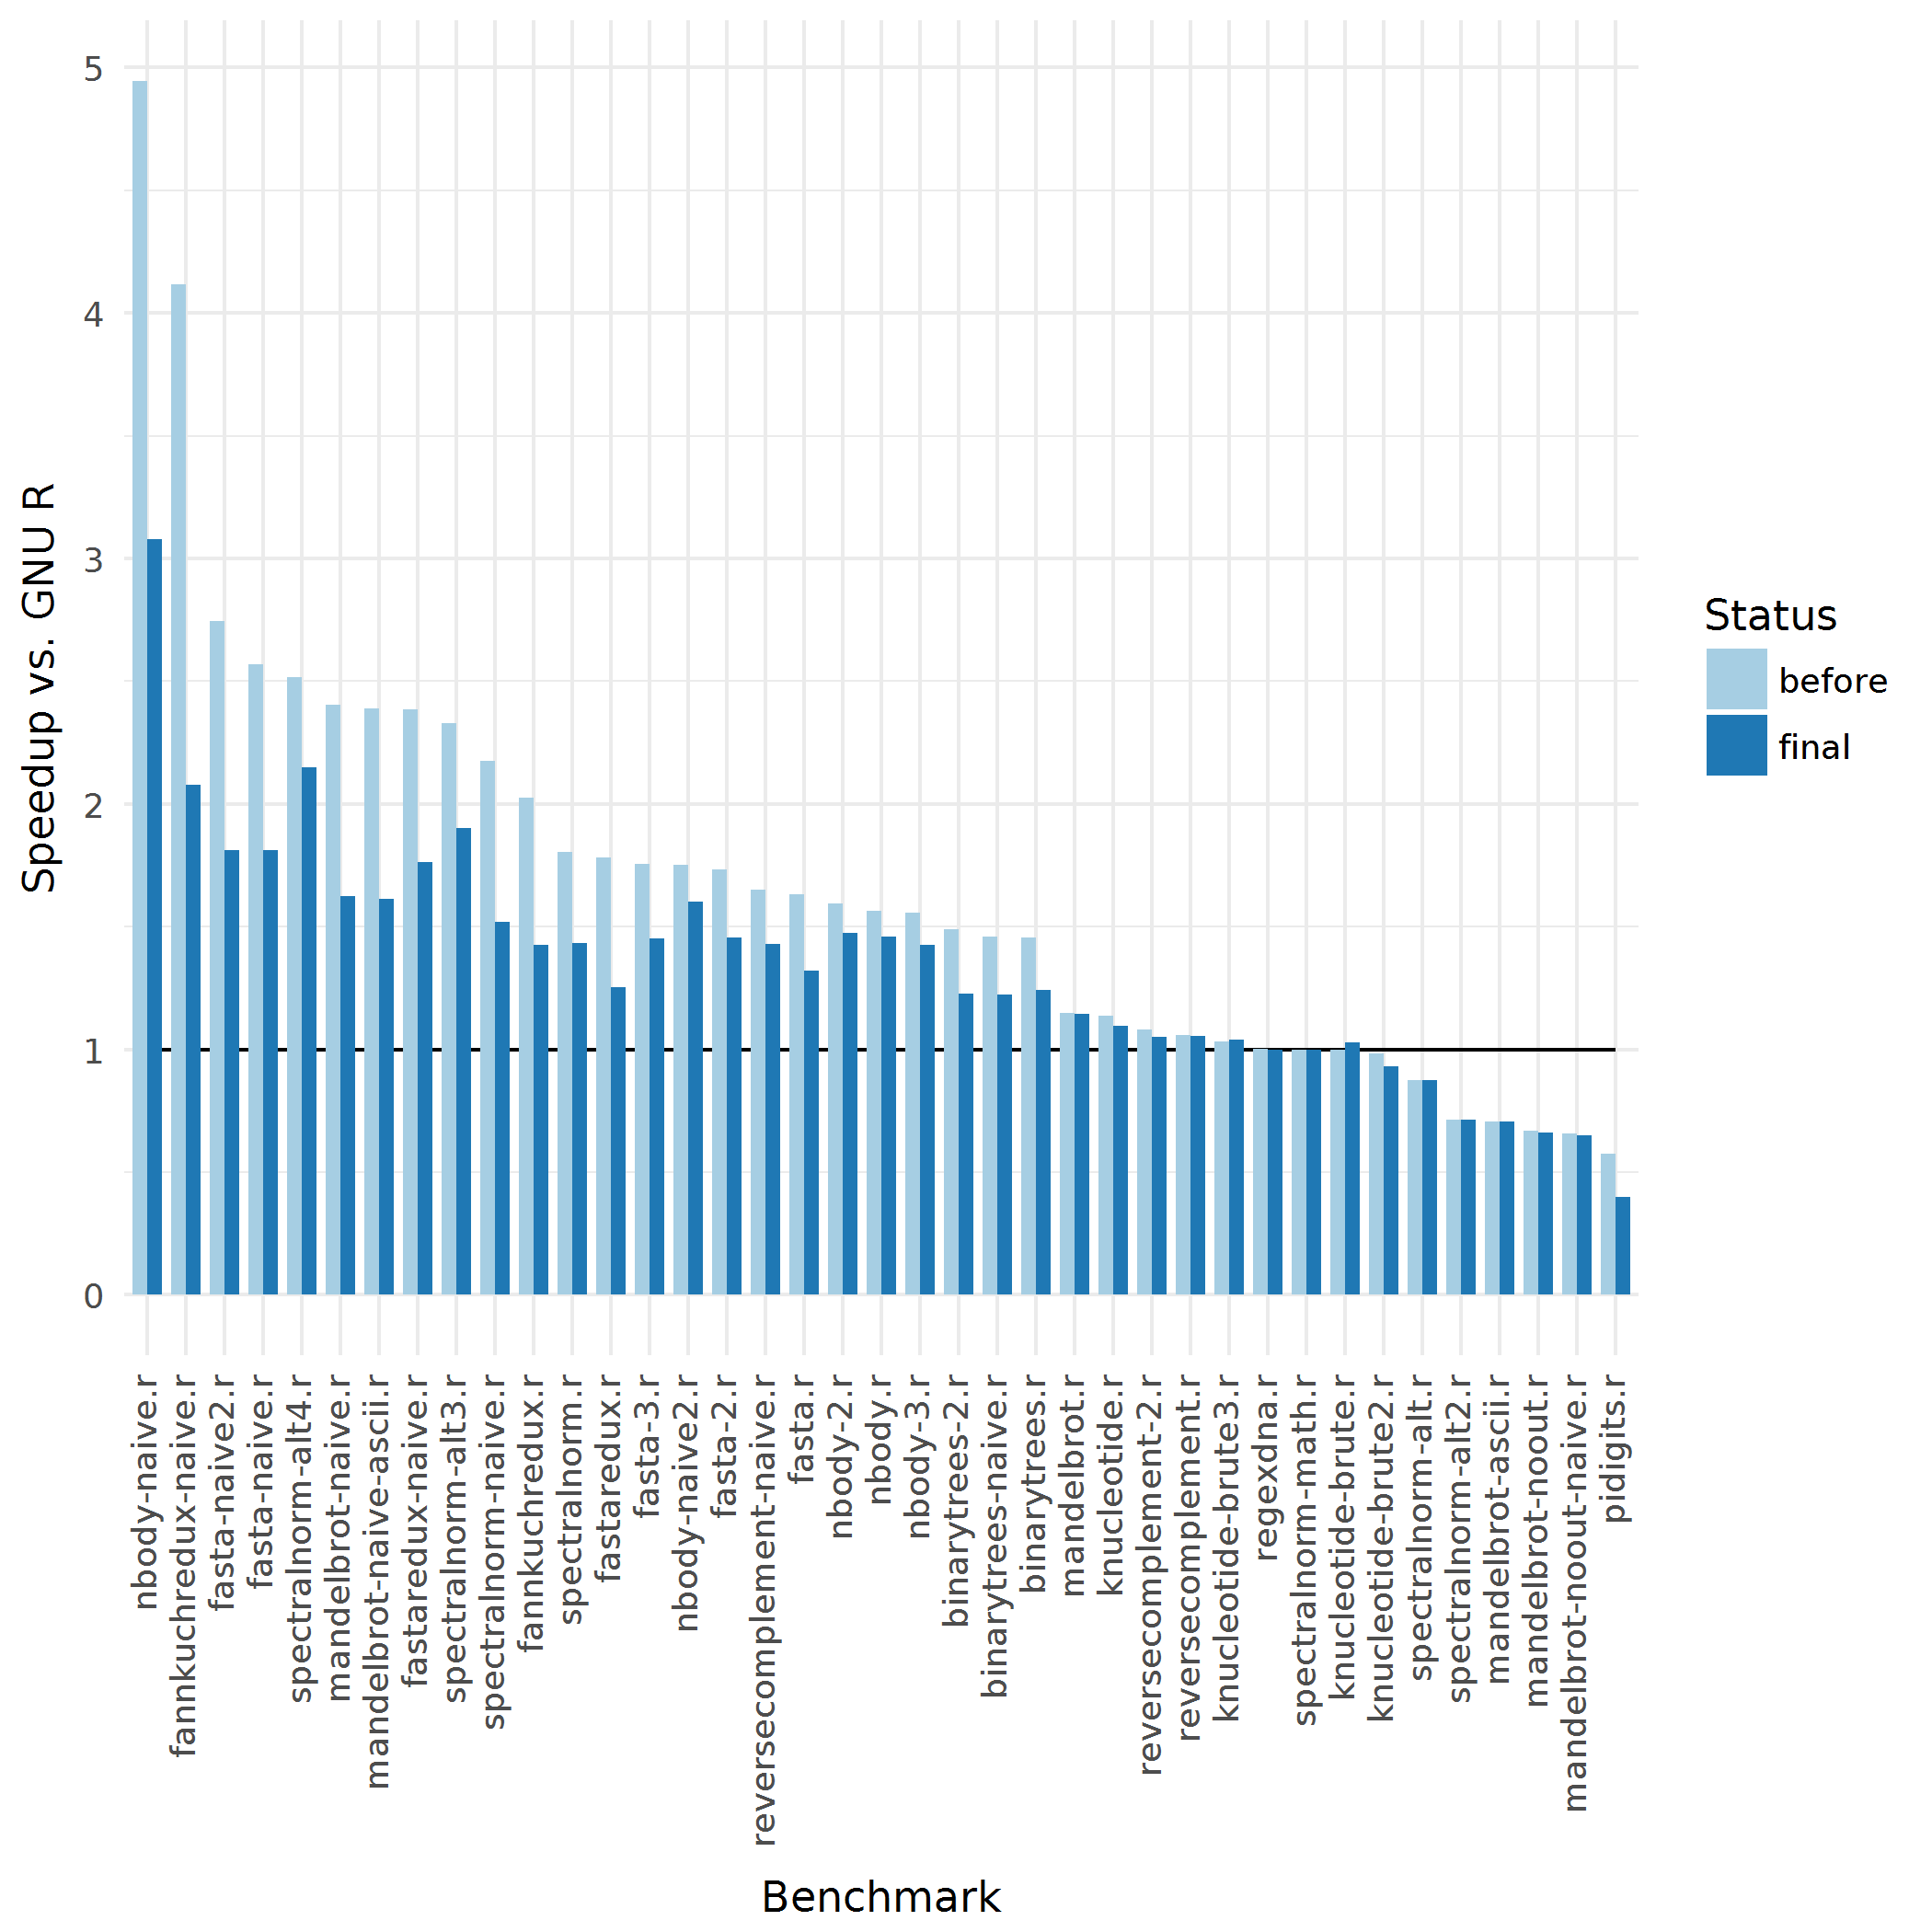
\includegraphics[width=\linewidth]{images/overall}}
\end{figure}

The lighter color refers to the state before anything was done, the darker after all the changes described in chapter \ref{improvements}.

The speedups are computed relative to the running time of GNU R byte-compiled code, which was normalized to 1 (this is indicated by the solid black line).

It can be clearly seen that the most speedup was gained in the naive implementations.

Overall, an average slowdown of about 1.678 against GNU R was lowered to about 1.336.
